 \chapter{Evaluation}\label{\positionnumber}
 As briefly mentioned in \fullref{2}, different algorithms yield different clusterings as well as the same clustering with different features and parameters yields different clusterings. Thus in order to find a suitable taxonomy extraction method for the property graph model the following steps are subsequently performed:
\begin{enumerate}
    \item Algorithm Selection: Find a suitable clustering algorithm that produces a taxonomy using a minimal feature vector and different parameters to cover the space of algorithms and parameters as extensively as feasible.
    \item Feature Vector Extension: Find a suitable feature vector that also leverages the graph structure.
\end{enumerate}
In the subsequent sections, the methods and steps taken is described for each of the two steps.
 Each step has its own requirements and objectives that are addressed in the subsequent sections, but both follow the same pipeline depicted in \fullref{fig:pipeline}. \\


\section{Tag-based clustering}\label{\positionnumber}
Tag-based clustering was mainly applied in order to probe a range of different algorithms.
The selection of a fitting algorithm has three main requirements:
\begin{itemize}
    \item Memory usage: Databases need a certain amount of memory to work, so the clustering algorithm must not use all memory to cluster data. That is the memory complexity shall be as low as possible
    \item Run time: The algorithm needs to have a decent run time complexity or must provide possible optimizations to scale it to large and very large data sets (i.e.~millions of nodes, tens of millions of edges).
    \item Adaptive to nominal and numeric data: Most databases support a couple of data types, that may be summarized as either nominal (string, characters, Boolean, $\dots$) or numeric (integer, long, floats, $\dots$), i.e.~the clustering algorithm needs to be able to support both kinds of data.
    \item Noise detection and tolerance: As there are frequently missing fields in data records the clustering algorithm should be tolerant to noise and detect noisy instances.
\end{itemize}
 In order to evaluate the so extracted taxonomy, a way of measuring the deviation from the ground truth is needed. The Tree Edit Distance is a measure defined as the minimum cost sequence of edit operations to a tree $T$ to transform it to another tree $T'$~\cite{Tai:1979:TCP:322139.322143}. A computationally more efficient and less memory consuming implementation is APTED by Pawlik et al~\cite{pawlik2016tree}, which is used for evaluation. The visualization provides illustrations of the dendrogram, the taxonomy, the flat clusters and the resulting tree edit distance.

\subsection{Setup}
\subsubsection{Data}\label{\positionnumber}
Inspired by the example given in \fullref{4.1} a synthetic data set is generated, that constructs tag sets yielding a homogeneous taxonomy with a user-defined height and width when extracting the taxonomy by hand. The height is the number of levels in the hierarchy and the width is the number of children each inner node has. This allows to measure the extracted hierarchy against a simple ground truth. \\
Data sets are by nature incomplete and noisy due to measurements or human errors.
So the data generator shall also be able to introduce noise, i.e.~to add, remove or alter labels in the label set of an object in order to measure the robustness of the taxonomy extraction method. 
An example of the generated data is shown in \fullref{tab:datagen}.
\begin{table}[htp]
     \centering
     \begin{tabular}{c c} \toprule
            Node.name & Node.labels \\ \midrule
            0 & l0, l00 \\ 
            1 & l0, l01 \\ 
            2 & l0, l02 \\ 
            3 & l1, l10 \\ 
            4 & l1, l11 \\ 
            5 & l1, l12 \\
            6 & l2, l20 \\ 
            7 & l2, l21 \\ 
            8 & l2, l22 \\ \bottomrule
        \end{tabular}
    \caption{A sample of generated data for parameters height = 2, width = 3 and noise = 0 }
    \label{tab:datagen}
\end{table}{}

\noindent Synthetic data provides fine grained control over noise and a ground truth to compare against. The parameters for height and width given in \fullref{tab:synthetic_params} are used for generation, where the height defines the number of levels in the resulting hierarchy and the width describes the number of children that each non-leaf node has. For each of them $0\%$, $5\%$, $10\%$, $20\%$, $33\%$ noise is applied. This is done for each number of samples specified in the \fullref{tab:synthetic_params}.
\begin{table}[htp]
     \centering
     \begin{tabular}{|c|c|c|} \hline
            No. Samples & Width & Depth \\ \hline \hline
            243 & 3 & 5 \\ \hline
            512 & 8 & 3 \\ \hline
            1024 & 4 & 5 \\ \hline
            1331 & 11 & 3 \\ \hline
            1728 & 12 & 3 \\\hline
            2197 & 13 & 3 \\ \hline
            2401 & 7 & 4 \\ \hline
            3125 & 5 & 5 \\ \hline
            4096 & 4 & 6 \\ \hline
            6561 & 9 & 4 \\ \hline
        \end{tabular}
    \caption{The parameters used during evaluation in the synthetic data generator.}
    \label{tab:synthetic_params}
\end{table}{}

\subsubsection{Implementation}
In order to probe as many algorithms as possible and in a representative way, state of the art implementations of scikit-learn~\cite{scikit-learn} and PyClustering have been used. Overall 16 different clustering algorithms have been tried, where only 8 of them are described in this thesis for the sake of brevity. During the implementation and experimentation the author found and fixed a bug in the widely used scikit-learn package. As most of the algorithms require parameters a parameter optimization technique was applied namely random search, with the silhouette coefficient as optimization criterion. In order to use the random search --- whose implementation is using the sklearn API --- with PyClustering, a wrapper around the algorithms of the latter was implemented. For conceptual clustering the TRESTLE algorithm from the concept formation package was used, that is an extension of Cobweb that tries to rename variables and restructure data to maximize the category utility when fitting it to the root node. \\

\noindent The pipeline was then executed on a machine with two (dual slot) 64-bit AMD EPYC 7531 16 core processors, clocked at 2.4GHz with 512GiB 2666MHz DDR4 RAM, an Intel 660P NVMe SSD running 64-bit Linux 4.15 (Ubuntu). Regarding Python the Anaconda distribution, version 1.7.2 implementing Python 3.7.3 was used, along with scikit-learn 0.22 and PyClustering 0.9.2.

\subsection{Results}\label{\positionnumber}
 The run time comparison of the algorithms described in \fullref{3} is shown in \fullref{fig:rt}. 
 \begin{figure}
\centering
\begin{tikzpicture}
    \begin{axis}[
        title=Runtime Results,
        width=0.5\textwidth,
        legend pos=outer north east,
        legend style={draw=none},
        axis lines = left,
        ymax = 1000.0,
        xlabel = Samples,
        ylabel = Runtime in s,
        grid=major,
        legend entries={DBSCAN,HDBSCAN,k-Means, OPTICS, RobustSingleLinkage, SingleLinkage, Trestle, TTSAS},
        %xtick=data
    ]
        \addplot [red, mark=x] file {data/part1/runtime/synth_DBSCAN_rt.dat};
        \addplot [blue, mark=square] file {data/part1/runtime/synth_HDBSCAN_rt.dat};
        \addplot [green, mark=*] file {data/part1/runtime/synth_KMeansWrapper_rt.dat};
        \addplot [black, mark=triangle] file {data/part1/runtime/synth_OPTICS_rt.dat};
        \addplot [cyan, mark=diamond] file {data/part1/runtime/synth_RobustSingleLinkage_rt.dat};
        \addplot [teal, mark=o] file {data/part1/runtime/synth_SingleLinkage_rt.dat};
        \addplot [brown, mark=square*] file {data/part1/runtime/synth_Trestle_rt.dat};
        \addplot [magenta, mark=+] file {data/part1/runtime/synth_TTSASWrapper_rt.dat};
    \end{axis}
\end{tikzpicture}
\caption{Run time comparison of the different algorithms discussed.} \label{fig:rt}
\end{figure}

\noindent First of all some of the search spaces of the parameter optimization got limited due to performance issues (e.g. when an algorithm ran for 10 hours+ with a sample size lower than 5000). More concretely there were two such algorithms namely OPTICS and TTSAS. From an algorithmic point of view the repeated neighbourhood queries for different $\epsilon$ values impose a high linear factor, especially when choosing an epsilon value close to 1 when using Jaccard distance. Thus the maximal considered neighbourhood region was $\epsilon = 0.5$. Similarly for TTSAS, if the thresholds are too far away from each other, both too low or too high (too high means the higher threshold is greater than one and the lower close to 1), the run time degenerates to cubic and the results are rather poor. Thus the thresholds distributions were uniform between $[0.4, 0.75]$ and $[0.75, 1]$. Single Linkage has the highest run time, but sometimes intersects other algorithms, which is surprising given the fact that it has the highest computational complexity of all the methods. When investigating the implementation, it becomes clear that single linkage has the most mature and optimized implementation using Cython (that is C bindings) resulting in faster execution times for some corner cases. Robust Single Linkage performs better in most cases and one can see, that Robust Sinlge Linkage also bounds HDBSCAN as its most computationally intensive part. TTSAS and k-Means perform well for small sample sizes, but do not scale too well to larger ones. In case of TTSAS the experiment with 6561 samples resulted in a run time of approximately 3400s which is probably due to sub-optimal thresholds. OPTICS is always lower bounded by DBSCAN and upper bounded by HDBSCAN. DBSCAN is the most basic variant of the considered density-based approached, thus has to lowest run time for all larger sample sizes. Trestle performs similar to HDBSCAN and Robust Single Linkage. \\


\noindent As the resulting tree edit distance correlates with the tree size and depth (in a larger tree there are more possible edits and more possible non-matching branches when inferring a tree), there are overall 3 visualizations, showing the tree edit distance depending on the introduced noise: 
\begin{itemize}
    \item \fullref{fig:ted4096} for a 4096 samples so for a hierarchy with depth 6 and width 4
    \item \fullref{fig:ted6561} for 6561 samples that is for a hierarchy with depth 4 and width 9
    \item \fullref{fig:tednorm} shows the averaged values, i.e.~$\frac{\text{Tree Edit Distance}}{|\text{samples}|}$ as function of noise independent of depth %% Averaged
\end{itemize}

 \begin{figure}
\centering
\begin{tikzpicture}
    \begin{axis}[
        title=Qualitative Results,
        width=0.3\textwidth,
        legend pos=outer north east,
        legend style={draw=none},
        axis lines = left,
        xlabel = Noise,
        ylabel = Tree Edit Distance,
        grid=major,
        legend entries={DBSCAN,HDBSCAN,k-Means, OPTICS, RobustSingleLinkage, SingleLinkage, Trestle, TTSAS},
        %xtick=data
    ]
        \addplot [red, mark=x,samples=5] file {data/part1/ted/DBSCAN_ted_4096.dat};
        \addplot [blue, mark=square, samples=5] file {data/part1/ted/HDBSCAN_ted_4096.dat};
        \addplot [green, mark=*, samples=5] file {data/part1/ted/KMeansWrapper_ted_4096.dat};
        \addplot [black, mark=triangle, samples=5] file {data/part1/ted/OPTICS_ted_4096.dat};
        \addplot [cyan, mark=diamond, samples=5] file {data/part1/ted/RobustSingleLinkage_ted_4096.dat};
        \addplot [teal, mark=o, samples=5] file {data/part1/ted/SingleLinkage_ted_4096.dat};
        \addplot [brown, mark=square*, samples=5] file {data/part1/ted/Trestle_ted_4096.dat};
        \addplot [magenta, mark=+, samples=5] file {data/part1/ted/TTSASWrapper_ted_4096.dat};
    \end{axis}
\end{tikzpicture}
\caption{Tree Edit Distance per noise level for 4096 samples} \label{fig:ted4096}
\end{figure}

\begin{figure}
\centering
\begin{tikzpicture}
    \begin{axis}[
        title=Qualitative Results,
        width=0.3\textwidth,
        legend pos=outer north east,
        legend style={draw=none},
        axis lines = left,
        xlabel = Noise,
        ylabel = Tree Edit Distance,
        grid=major,
        legend entries={DBSCAN,HDBSCAN,k-Means, OPTICS, RobustSingleLinkage, SingleLinkage, Trestle, TTSAS},
        %xtick=data
    ]
        \addplot [red, mark=x, samples=5] file {data/part1/ted/DBSCAN_ted_6561.dat};
        \addplot [blue, mark=square,  samples=5] file {data/part1/ted/HDBSCAN_ted_6561.dat};
        \addplot [green, mark=*,  samples=5] file {data/part1/ted/KMeansWrapper_ted_6561.dat};
        \addplot [black, mark=triangle,  samples=5] file {data/part1/ted/OPTICS_ted_6561.dat};
        \addplot [cyan, mark=diamond,  samples=5] file {data/part1/ted/RobustSingleLinkage_ted_6561.dat};
        \addplot [teal, mark=o,  samples=5] file {data/part1/ted/SingleLinkage_ted_6561.dat};
        \addplot [brown, mark=square*,  samples=5] file {data/part1/ted/Trestle_ted_6561.dat};
        \addplot [magenta, mark=+,  samples=5] file {data/part1/ted/TTSASWrapper_ted_6561.dat};
    \end{axis}
\end{tikzpicture}
\caption{Tree Edit Distance per noise level for 6561 samples} \label{fig:ted6561}
\end{figure}

 \begin{figure}
\centering
\begin{tikzpicture}
    \begin{axis}[
        title=Qualitative Results,
        width=0.3\textwidth,
        legend pos=outer north east,
        legend style={draw=none},
        axis lines = left,
        xlabel = Noise,
        ylabel = $\frac{\text{Tree Edit Distance}}{|\text{samples}|}$,
        grid=major,
        legend entries={DBSCAN,HDBSCAN,k-Means, OPTICS, RobustSingleLinkage, SingleLinkage, Trestle, TTSAS},
        %xtick=data
    ]
        \addplot [red, mark=x,samples=5] file {data/part1/ted/DBSCAN_ted_norm.dat};
        \addplot [blue, mark=square, samples=5] file {data/part1/ted/HDBSCAN_ted_norm.dat};
        \addplot [green, mark=*, samples=5] file {data/part1/ted/KMeansWrapper_ted_norm.dat};
        \addplot [black, mark=triangle, samples=5] file {data/part1/ted/OPTICS_ted_norm.dat};
        \addplot [cyan, mark=diamond, samples=5] file {data/part1/ted/RobustSingleLinkage_ted_norm.dat};
        \addplot [teal, mark=o, samples=5] file {data/part1/ted/SingleLinkage_ted_norm.dat};
        \addplot [brown, mark=square*, samples=5] file {data/part1/ted/Trestle_ted_norm.dat};
        \addplot [magenta, mark=+, samples=5] file {data/part1/ted/TTSASWrapper_ted_norm.dat};
    \end{axis}
\end{tikzpicture}
\caption{Tree Edit Distance per noise level divided by sample size} \label{fig:tednorm}
\end{figure}

\noindent One can clearly see, that single linkage is by design not able to group objects that have equivalent attributes in one cluster in a single step, but rather in subsequent steps, resulting in a very high tree edit distance. Robust Single Linkage provides great improvements over classic Single Linkage, as it allows merging multiple objects at once and only merges multiple objects when appropriate. The density-based methods are quite similar when it comes to the tree edit distance, i.e.~very robust to noise, but only in rare cases exact. k-Means is always worse than the density-based approach in terms of the tree edit distance, like TTSAS even tough TTSAS is able to reach similar TED scores as the density-based approach. Trestle is the only algorithms whose performance decreases with the introduced noise and the only algorithm that improves with the height of the ground truth hierarchy. This is especially noticable when comparing \fullref{fig:ted4096} with \fullref{fig:ted6561}, where the point of intersection between Trestle and the density-based approaches is at a higher noise level compared due to 2 more steps in the hierarchy as compared to the latter figure where this intersections happens almost at 0 nosie. This is due to the fact that it is the only algorithm able to change the depth of the inferred hierarchy through out the whole processing step. 

\subsection{Discussion}\label{\positionnumber}
The results with respect to time only focus on the clustering time itself. When looking at multi-phase approaches and robust single linkage, we have to keep in mind that those algorithms have parameters that need to be inferred to obtain meaningful results. Depending on the parameter space and the inference method this may take a dominant amount of time as each iteration in the inference process must use at least some representative sample of the data and execute the full algorithm on that. For example a randomized search samples parameters from used-defined distributions a pre-defined number of times and executes the algorithm on the whole data set to evaluate the results with respect to a user defined measure. This may result in factors of more than 100 for medium and large parameter spaces with non-trivial restrictions of the parameters. However note, that also the inference of parameters is of course highly dependent on an appropriate choice of the parameter distribution or restricted space (depending on inference methodology). That is the presented run times are not guaranteed to be globally optimal, but rather the local optimum found by the randomized search. \\
Additionally the vectorization of categorical attributes that is necessary for all algorithms besides Trestle --- or more generally conceptual clustering approaches --- uses additional space, that is equivalent to the number of distinct values of all attributes, what may grow relatively large. Although this amount of memory may be freed when the distance matrix is computed, one needs the memory for both the objects including vectorized attributes and the distance matrix. For large data sets this is infeasible and provides little possibilities for optimization. One would be explicit swapping when iterating over the elements during distance computation, so that at any time only a part of the matrix would be in main memory as well as only a couple of objects at a time. This may be achieved using a database and an implementation that does I/O similarly to the two-way merge sort algorithm. \\
Another issue is that of noisy data sets. When there is too much noise, the intersection of the attributes in a cluster may be empty, resulting in unusable object descriptions and non-sense hierarchies that get extracted. Additionally there is the need to flatten the dendrogram that is produced during Single Linkage Clustering, which can only unify subsequent merges but not restructure the merges in general. \\
Some of the so far evaluated approaches may be applied to the graph-aware pipeline, when integrating them more closely with the memory optimization facilities of a database in mind and further refinements, like introducing a fuzzy intersection to describe cluster representatives in the multi-phase approach.
        

\section{Graph-aware clustering of Nodes}\label{\positionnumber}
Conceptual clustering provides a lot of useful traits for this application: 
\begin{itemize}
    \item Parameter-free: As Cobweb does not need additional parameters, there is no need to tune those i.e.~the algorithm fits to the data by its' own means in theory.
    \item Memory: It is incremental and thus uses in the most inefficient implementation $\mathcal{O}(n)$ memory. Does not require vectorization or similar things.
    \item Computation: Generally Conceptual clustering is able to integrate a node in logarithmic time with respect to the number of already incorporated instances, but also requires  $B + 4 \cdot 3B \cdot A \cdot 2V$ floating point computations, which may grow very large, depending on the number of attributes and values. Finding an objective function that is rank-preserving and uses less computations, reducing the number of occasions where the objective function is computed and a way to only select the most discriminating attributes provides means for optimization of the computational complexity.
    \item Probabilistic concept descriptions: The problem of an empty intersection is overcome by using probabilistic concept descriptions, that may also provide further helpful information in query optimization.
    \item Hierarchical: Producing not a dendrogram but rather a data driven hierarchy of variable branching factor, that is no post-processing is needed.
    \item Existing extension to mixed data without additional memory or computational complexity. \\ 
    In contrast to what McKusick et al. reports (``[...] summing together terms from both forms of the equation works well in domains with mixed data.``)~\cite{mckusick1990cobweb}, mixed data processing was dominated by numeric values, thus a constant bias was added to the denominator of the equation for continuous values in \fullref{3.4.2}.
\end{itemize}
For this reason Cobweb is used for the evaluation of the graph-aware pipeline. Density-based algorithms in combination with robust single linkage may provide superior robustness and faster run times, but also require further adaptions which introduce additional degrees of freedom. As we want to experiment with different feature vectors this is undesirable here and we stick with the maybe sub-optimal but more convenient cobweb algorithm. \\

\subsection{Setup}\label{\positionnumber}
\subsubsection{Data}
\fig{img/ldbc_snb.png}{ldbc}{The schema for the LDBC SNB benchmark}{0.7}
The Linked Data Benchmark Council (LDBC) consists of a group of industrial and academic organizations that research on databases e.g. the Technische Universitaet Muenchen, Neo4j or the Vrije Universiteit Amsterdam. The LDBC social network benchmark aims at fulfilling the following requirements:
\begin{itemize}
    \item Cover most demands that arise when managing data
    \item Modular structured, i.e.~may be broken into pieces without large overhead
    \item Balanced selection of challenges
    \item Modest implementation cost
    \item Reproducibility and documentation
\end{itemize}
The synthetic data set that is generateable using the software provided by the LDBC mimics a social network that follows the schema in \fullref{fig:ldbc}. To ensure realism the authors modeled data link distributions as found in real world social networks like Facebook and provided attribute values found in DBpedia. They also pay attention to regularities like homophily in the links of social networks, i.e.~in a social context there tend to be more connections between people that behave similar and have similar interests. To ensure scaling ability of the generation process, it is implemented using the MapReduce paradigm.
\noindent The LDBC SNB dataset is used to probe the pipeline as some sort of ground truth is available, even though this ground truth only considers node labels in the sense of a label in Neo4j rather than similar instances. The cardinalities of instances in the database is a dominant factor for deriving such a hierarchy. For example consider a sample size of 10000. If 9950 of 10000 samples are instances with the node label message, the output of a taxonomy will mainly provide characteristics of nodes with those labels while nodes with other labels are a minority and may even be classified as noise.
  Additionally the yelp data set is used as an example for a not graph but rather ``object-oriented`` or property-oriented data set. 
  One experiment uses the New York Road Net data set provided by the 9th DIMACS shortest path challenge to demonstrate the pipeline on a less complex and spatially graph-oriented data set~\cite{9thDIMACSImplementationChallengeShortestPaths-2010-06-14}.
  
\subsubsection{Pre-Processing}
Cobweb is able to deal with character strings by design, while all other clustering algorithms introduced in \fullref{3} require dictionary vectorization as pre-processing step.
  \noindent A number of different combinations of the following features has been used:
\begin{itemize}
    \item the labels of the nodes $V, L, f_l$ 
    \item the properties of the nodes
    \item per node structural features of the underlying graph that is the node degree, the average neighbour degree, the number of nodes incoming to the ego net and the number of nodes outgoing from the ego net
    \item the characteristic set of a node, that is the set of all relation types associated with this node 
\end{itemize}
The node labels have always been used. For the latter three features, all variations (i.e.~the labels plus one element of the power set) have been tried. \\
  
  \subsubsection{Implementation}
  In order to integrate the proposed method with Neo4j and potentially move it to a deeper level in the architecture of the database it was implemented as a Cypher procedure so that it complies with the internal API of Neo4j and can be called from the query language Cypher. The implementation of Cobweb was done by the author from scratch as well as all feature extraction traversals of the graph, besides the node degree. \\
The implementation of Cobweb uses the adjusted category utility from ~\cite{mckusick1990cobweb} and an unbiased and numerically stable algorithm for computing mean and variance, namely Chan's Algorithm~\cite{chansAlgo} as proposed by MacLellan et al~\cite{maclellan2016trestle}.
For testing purposes, an annotation-based database setup and import framework was written, provided by Manuel Hotz and refined by the author. \\
In order to boost the computational performance a multi-threaded version was implemented but yielded high contention that cancelled the concurrency gains in Cobweb. There is further space for optimization regarding memory access patterns, caching and storing intermediate values to avoid the computation of the same value over and over again. \\

The pipeline was again executed on a machine with two (dual slot) 64-bit AMD EPYC 7531 16 core processors, clocked at 2.4GHz with 512GiB 2666MHz DDR4 RAM, an Intel 660P NVMe SSD running 64-bit Linux 4.15 (Ubuntu). Regarding Java the OpenJDK distribution, version 11.0.4 was used, along with Neo4j 3.5.3.

\subsection{Results}\label{\positionnumber}
In \fullref{fig:ldbctree} the ground truth label hierarchy is shown.
\begin{figure}
    \centering
    \begin{figure*}[t]
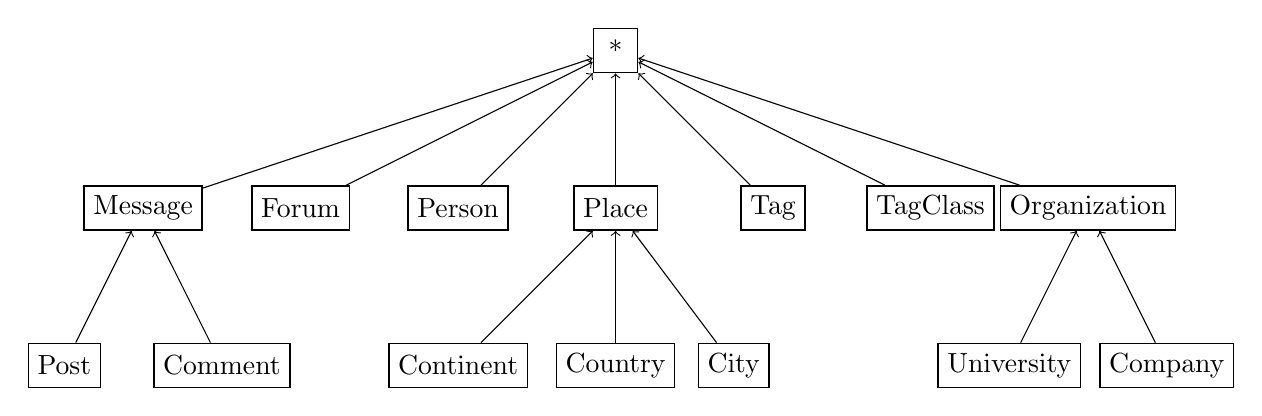
\begin{tikzpicture}
\node[draw=black,minimum size = 16pt,line width = 0.5pt,] at (0, 0)  		(ROOT)	{*};
\node[draw=black,minimum size = 16pt,line width = 0.5pt,] at (-6, -2) 	(N1) 	{Message};
\node[draw=black,minimum size = 16pt,line width = 0.5pt,] at (-4, -2) 	(N2)	{Forum};
\node[draw=black,minimum size = 16pt,line width = 0.5pt,] at (-2, -2) 	(N3) 	{Person};
\node[draw=black,minimum size = 16pt,line width = 0.5pt,] at (0, -2)  	(N4) 	{Place};
\node[draw=black,minimum size = 16pt,line width = 0.5pt,] at (2, -2)  	(N5) 	{Tag};
\node[draw=black,minimum size = 16pt,line width = 0.5pt,] at (4, -2)  	(N6) 	{TagClass};
\node[draw=black,minimum size = 16pt,line width = 0.5pt,] at (6, -2)  	(N7)	{Organization};
\node[draw=black,minimum size = 16pt,line width = 0.5pt,] at (-7, -4) 	(N11) 	{Post};
\node[draw=black,minimum size = 16pt,line width = 0.5pt,] at (-5, -4) 	(N12) 	{Comment};
\node[draw=black,minimum size = 16pt,line width = 0.5pt,] at (-2, -4)  	(N41) 	{Continent};
\node[draw=black,minimum size = 16pt,line width = 0.5pt,] at (0, -4)  	(N42) 	{Country};
\node[draw=black,minimum size = 16pt,line width = 0.5pt,] at (1.5, -4)  	(N43) 	{City};
\node[draw=black,minimum size = 16pt,line width = 0.5pt,] at (5, -4)  	(N71)	{University};
\node[draw=black,minimum size = 16pt,line width = 0.5pt,] at (7, -4)  	(N72)	{Company};
\draw[<-] (ROOT) -- (N1);
\draw[<-] (ROOT) -- (N2);
\draw[<-] (ROOT) -- (N3);
\draw[<-] (ROOT) -- (N4);
\draw[<-] (ROOT) -- (N5);
\draw[<-] (ROOT) -- (N6);
\draw[<-] (ROOT) -- (N7);
\draw[<-] (N1) -- (N11);
\draw[<-] (N1) -- (N12);
\draw[<-] (N4) -- (N41);
\draw[<-] (N4) -- (N42);
\draw[<-] (N4) -- (N43);
\draw[<-] (N7) -- (N71);
\draw[<-] (N7) -- (N72);
\end{tikzpicture}
\caption{Label hierarchy for the SNB database.}
\end{figure*} 

    \caption{Ground truth label hierarchy for the LDBC SNB data set}
    \label{fig:ldbctree}
\end{figure}{}
The trees visualized in the following section are the label hierarchies that were inferred with generated abstract labels. That means the labels in the trees shown as result have no semantic meaning and are solely there to reference the table describing the same concept as the node. Also the root of the tree is always called ``Root`` as it always contains an aggregation of all values present in the feature vector for all incorporated nodes. The tables for all concepts shown in the trees can be found in the appendix. An exemplar table is shown in \fullref{lldbccnl0}
As the trees get relatively large due to saving each instance as an extra node, the results are cut at the second level of the tree which is mostly sub-optimal. This is a similar problem as the one of single linkage, that is further addressed in extensions of the Cobweb algorithm e.g. in \cite{classit, thompson1989incremental} and others.
We shall visually inspect differences, as due to the above mentioned difficulties, the tree edit distance may be closer to the ground truth even tough the learned concepts aren't. 
Also some values in the concept description tables are not visualized, as the tables get very large (more than 100 rows, some values wider than what fits on A4 paper). 
Many of the trees contain the desired concepts, but at levels that are not always the same, i.e.~there is no level in the tree that contains optimal concepts for all branches. 
For instance as the ratio of persons to messages is very low, the desired concept of persons may be at a very low level and the desired concept for messages is at a rather high level in the tree. 
That is concepts with high support are at a high level in the tree, while concepts with low support are at lower levels. For all the data sets a sample size of 2000 nodes and all relationships connecting to those nodes was used. \\

\paragraph{Labels Only}
When only taking the node labels into account on the LDBC SNB data set, the algorithm splits at the first level all Comments (which are also messages) and then all posts at the next level. This is also due to the cardinality of the label sets. The fact that both l0 and l10 conatin the label message is probably due to order effects described by Fisher in more detail~\cite{Fisher1987}. All other labels are present at such low total probabilities, that the split that separates those eventually is at a deeper level in the tree. The tree is shown in \fullref{fig:lldbctree} and an example for a concept description table can be found in \fullref{l0ex}. \\

\begin{figure}[htp]
    \centering
    \begin{forest}
[Root
	[l0 
		[l00 
]		[l01 
]		[l02 
]]	[l1 
		[l10 
]		[l11 
]]]
\end{forest} \\
    \caption{Inferred Label Hierarchy with labels only}
    \label{fig:lldbctree}
\end{figure}{}
\begin{table}[H] 
  \centering 
 \begin{longtable}{|c|c|c|c|c|} \hline 
Attribute & ValueType & Value & Probability & Occurences \\ \hline 
\multirow{2}{*}{Labels} & Nominal & Message & $1.0000$ & $1289$ \\ \cline{2-5} 
 & Nominal & Comment & $1.0000$ & $1289$ \\ \hline 
 \captionsetup{position=top}
 \caption{Example concept description for node l0: P(node) = 0.6445, Count = 1289}\label{l0ex}
\end{longtable}
 \end{table} 

If the label distribution only consists of one equally probable label for all nodes there is no valuable information that can be used to cluster the data instances, thus the tree is made up of a single root node and no information is gained. An example here fore is the yelp data set with properties to store all information when it is clustered using only the label sets. That is for all nodes ``Business`` so there is only one concept containing all nodes. \\
 
 \paragraph{Labels and Node Properties}
\begin{figure}[htp]
    \centering
    \begin{forest}
[Root
	[l0 
		[l00 
]		[l01 
]		[l02 
]]	[l1 
		[l10 
]		[l11 
]]]
\end{forest}
    \caption{Inferred Label Hierarchy for the LDBC SNB data set with labels and properties as the feature vector}
    \label{fig:lpldbctree}
\end{figure}{}
The first three levels of the generated tree is shown in \fullref{fig:lpldbctree}. When using the properties additionally to the set of labels, a sub-tree is appended at l0 splitting nodes that have labels message and comment further into messages of created with different browsers. The sub-tree starting at l1 is very similar to the one with only labels: It splits into nodes having the labels message and post and those having anything else but in contrast to before still contains nodes having the labels message and post. The unclean split is due to the extra noise introduced with the presence of the properties. As there are a lot of properties, the predictiveness of some properties (e.g. the id, what browser was used, the creation date) weakens the effect of the label predictiveness and thus introduces additional noise. \\

\begin{figure}[htp]
    \centering
    \input{data/part2/lp/yelp_oo_0Tree.tex}
    \caption{Inferred Label Hierarchy for the property-oriented Yelp data set with labels and properties as the feature vector}
    \label{fig:lplyelpootree}
\end{figure}{}
In the previous paragraph we noticed, that a data set with only one equi-probable label for all nodes contains no information. If a data set has node properties, adding those to the feature vector enables the use of clustering methods to extract concepts. The first three levels of the generated tree is shown in \fullref{fig:lplyelpootree}. Depending on how predictive the properties are and in how many directions they are, the resulting hierarchy may be clean but is mostly rather messy: For instance the property-based Yelp data set contains attributes describing spatial features (the exact location including latitude, longitude, address, state, $\dots$), time based features (the opening hours), numeric and nominal ones (user-defined categories, price ranges, an average review score and a review count for example). Optimizing for those in common yields a mixture of the above which introduces a lot of noise. Some semantically close instances are in different concept classes as their spatial position differs completely, while some spatially and semantically close instances are in distinct groups due to different tags assigned (covering traits like WiFi, Parking, GoodForChildren). Extensions of the algorithm to deal with Spatial and Date-based values, to find correlations in the attribute-value distribution and to evaluate only the most salient and discriminative values or weighting, cleaning and projection of properties before clustering may provide further refinements to improve the result using properties in the feature vectors. \\

Considering a road network data set, with no node labels and no properties, there is no information to cluster the nodes with, that is this feature vector yields no information for such data sets. \\

\paragraph{Labels and Characteristic Sets}
\begin{figure}[htp]
    \centering
    \begin{forest}
[Root
	[l0 
		[l00 
]		[l01 
]		[l02 
]]	[l1 
		[l10 
]		[l11 
]]]
\end{forest} \\
    \caption{Inferred Label Hierarchy for the SNB data set with labels and the characteristic set as the feature vector}
    \label{fig:lcldbctree}
\end{figure}{}
Taking the characteristic set into account results in more information than with labels only but less noise than with the properties for most cases. Applied to the LDBC SNB data set, the concepts are similar to the ones created with labels only with some additions: l0 is again the concept that contains nodes with labels message and comment, but additionally separates between nodes that have relationships to tags, nodes that do rather not and a class where approximately two thirds of the nodes have tags. The latter one is probably created erroneously due to ordering effects. In the sub-tree of l1 again nodes with labels Message and Post are split from the rest of the nodes. There are actually two sub-concepts for nodes with labels Message and Post: One where there are mostly tagged answer posts, and one where the posts are not in reply to something and barely have tags. The first three levels of the generated tree is shown in \fullref{fig:lcldbctree}. \\

Again if we have no relationships as in the property-oriented yelp data set we gain no information by adding the characteristic set (as it is an empty set). Another case where no relevant information is gained is the case of a road network: Every node has edges with the relationship type ``ROAD``. That is all characteristic sets are exactly the same containing one element --- namely ``ROAD``. \\

\paragraph{Labels and Structural Features}
\begin{figure}[htp]
    \centering
    \begin{forest}
[Root
	[l0 
		[l00 
]		[l01 
]		[l02 
]]	[l1 
		[l10 
]		[l11 
]]]
\end{forest} \\
    \caption{Inferred Label Hierarchy for the SNB data set with labels and structural features as the feature vector}
    \label{fig:lsldbctree}
\end{figure}{}
Here the nodes are structured as with just the labels, but additionally in the sub-tree l0 there is a distinction between lower mean node degree, lower number of outgoing edges, higher average neighbour degree and higher mean node degree, higher number of outgoing edges, lower average neighbour degree. On the sub-tree of l1 there is again the nodes having the labels message and post and those having anything else split. This time the split provides additional relevant information: nodes with labels ``Message`` and ``Post`` have mostly a low degree and a lower number of edges outgoing from the ego net but a high number of edges incoming to the ego net and a high average neighbour degree, whereas nodes with other labels have on average a higher degree, more outgoing than incoming edges to the ego net and a lower average neighbour degree. The first three levels of the generated tree is shown in \fullref{fig:lsldbctree}. Note however, that more complex structural features can be extracted in order to extract more complex meaning from the data and that a different bias term as mentioned in the first paragraph of \fullref{5.2} may change the result significantly. That is if numeric values dominate the result, the influence that the labels (nominal values) have decreases in comparison to the structural features which are numeric. This also applies for properties (mixed) and the characteristic set (nominal). \\

\begin{figure}[htp]
    \centering
    \begin{forest}
[Root
	[l0 
		[l00 
]		[l01 
]]	[l1 
		[l11 
]]	[l2 
		[l20 
]		[l21 
]		[l22 
]		[l23 
]		[l24 
]]]
\end{forest} \\
    \caption{Inferred Label Hierarchy for the New York road network data set with labels and structural features as the feature vector}
    \label{fig:lsroadnetnytree}
\end{figure}{}
For the property oriented yelp data set we have again no meaningful information gain as it does not contain any relationships. \\

For the road network example the situation looks a bit different now: Crossings connecting many streets and those who only connect two streets are separated as well as streets in more or less dense networks. The sub-tree l0 contains all crossings having exactly 3 roads that are connected. It further sub-divides into crossings whose ego nets have between 17 (l03) and 23 (l01) incoming and outgoing roads. Sub-tree l1 contains all crossings that connect exactly 1 road (dead ends). Last but not least sub-tree l3 contains crossings connecting either 2 or 4 roads with 15 and 31 incoming and outgoing roads respectively. The first three levels of the generated tree is shown in \fullref{fig:lsroadnetnytree}.


\paragraph{Labels and mixtures of the other features}
\begin{figure}[htp]
    \centering
    \begin{forest}
[Root
	[l0 
		[l00 
]		[l01 
]		[l02 
]]	[l1 
		[l10 
]		[l11 
]]]
\end{forest} \\
    \caption{Inferred Label Hierarchy for the SNB data set with labels, structural features and the characteristic set as feature vector}
    \label{fig:lscldbctree}
\end{figure}{}
When taking labels, structural features and the characteristic set as the feature vector the resulting hierarchy is the same, if only the structure of the hierarchy is considered. The first three levels of the generated tree is shown in \fullref{fig:lscldbctree}. Semantically at the sub-tree l1 nodes with the labels Message and comment are split as for most of the example hierarchies before. The split happening after l1 separates nodes with a degree of exactly 3 (std is 0.027) from higher degree nodes with a mean degree of 9. This indicates the number of tags of the comment: The higher the degree, the more tags are attached, which is also visible from significant differences in the probabilities of the characteristic set containing the HAS\_TAG relationship ($99.5\%$ for the higher degree nodes versus $0.35\%$ for the lower degree nodes). The sub-tree l0 separates again the rest of the nodes and the children sub-divide into nodes with labels Message and Post (l01, l02) and the rest (l00). The concepts l01 and l02 separate posts with a high degree and a low degree indicating more or less tags and replies as with comments. This time the probabilities are $3,8\%$, $0.21\%$, $0\%$ versus $17\%$, $89.7\%$, $85.2\%$ for likes, tags and replies respectively. \\


\begin{figure}[htp]
    \centering
    \begin{forest}
[Root
	[l0 
		[l00 
]		[l01 
]		[l02 
]]	[l1 
		[l10 
]		[l11 
]]]
\end{forest} \\
    \caption{Inferred Label Hierarchy for the SNB data set with labels, node properties, structural features and the characteristic set as feature vector}
    \label{fig:lpscldbctree}
\end{figure}{}
Taking the properties additionally into account introduces more noise, that is more features of for which the information gain is unknown and might be negative (that is adding the information to the feature vector actually interferes with the algorithm's ability to extract the relevant concepts with the correct attribute value distribution from the underlying data distribution). The first three levels of the generated tree is shown in \fullref{fig:lpscldbctree}. Here l0 splits again between nodes with labels message comment but in the subsequent step the predictiveness of using a certain browser is maximized which is a characteristic of the data which does not carry any further information about structure and distribution of the data. In the other sub-tree again nodes with the labels message and post are split from the nodes containing all other labels. \\


\subsection{Discussion}\label{\positionnumber}
 None of the generated concepts or label hierarchies do match fully to the ground truth, but this is also not what is desired. Desired is to extract meaningful and representative concept classes that can be used to derive labels. For example the LDBC data set contains about $95\%$ nodes with the label ``Message`` and only a very small amount of nodes with the label ``Person``. Therefore it is representative to split at the first steps into ``Message and non-Message``-labled nodes as this is the major difference between the largest group of nodes in this data set and all the others. \\
 The results clearly indicate that there is no single feature vector which can be used to extract meaningful concepts from all data sets. For data sets not leveraging graph structures, the characteristic set and structural features contain no information like in the non-transformed yelp data set. For those which do not have properties attached to the data set, taking the properties into account yields no information. Road network data like the New York road net data set contain often no labels, that is taking the labels into account in the feature vector adds no information. \\
 On the other hand, adding the properties to the feature vector may introduce additional noise and actually disturb the derivation of meaningful concepts that represent the underlying distribution. \\
 Constructing the feature vector adaptively seems to be the only option resulting in a minimal and complete source of information on the data set. That is if there are no relations but properties, only the properties and eventually the labels when meaningful shall be used. On the other hand for data sets not containing properties, useful labels and more than one relationship type, structural features are the only usable feature that should be used and so on. \\
 Also extensions to the algorithms to make the procedure detect significant correlations, deal with temporal and spatial data types (and possibly others requiring special semantics to yield useful aggregations not considered here) and the ability to only use those attributes with the highest information gain. In general it seems that both a Bayesian and an information theoretic extension of the conceptual clustering framework may counter some of the problems. Applied to the other clustering algorithms such extensions would require additional pre-processing, for instance a sampling procedure to estimate correlations and to calculate the information gain for certain attributes or groups of correlated attributes. \\
 As the distributions that shall be learned are only constrained to model numeric values as Gaussians, there is no upper bound for the sample complexity, due to the no free lunch theorem. Further when loosening the Gaussian prior which has no concrete theoretical justification the space of possible distributions is unrestricted. 
